\documentclass{article}


\usepackage[]{geometry}

\usepackage{titling} % center cover page
\renewcommand\maketitlehooka{\null\vfill} % center cover page
\renewcommand\maketitlehookd{\vfill\null} % center cover page

\usepackage{tocloft} % add dots for sections in table of contents
\renewcommand{\cftsecleader}{\cftdotfill{\cftdotsep}} % add dots for sections in table of contents

\usepackage{hyperref} % make table of contents clickable
\hypersetup{ % remove default ugly look of links
	colorlinks,
	citecolor=black,
	filecolor=black,
	linkcolor=black,
	urlcolor=black
}

%\AddToHook{cmd/section/before}{\clearpage} % each section starts on new page

\usepackage{acronym} % acronyms

\usepackage{graphicx} % required to load images







\hypersetup{pdftitle={Web Applications Architecture - English}}
\hypersetup{pdfauthor={Spyros Alertas}}
\hypersetup{pdfsubject={Web Applications Architecture - Notes}}
\hypersetup{pdfkeywords={Web Applications Architecture, Database, Back End, API, Front End}}

\title{\bfseries{Web Applications Architecture}}

\author{Spyros Alertas}

\date{Created On: September 02, 2023\\Last Edit: \today}

% Hint: \title{whatever}, \author{who cares} and \date{whenever} could stand before or after the \begin{document} command BUT the \maketitle command MUST come AFTER the \begin{document} command!

\begin{document}


% cover page
\begin{titlingpage}
\maketitle
\end{titlingpage}


% table of contents
\tableofcontents


% all sections - main document content
\newpage
\section{Introduction}
\paragraph{} This document is a brief description of the main parts that compose a web application and some of the different choices we have for each of them.


\section{Main Parts of a Web Application}
\paragraph{} The main parts of a web application are:
\begin{itemize}
	\item \textbf{Database:} Responsible for the storage of data.
	\item \textbf{Back End:} Implements the business logic.
	\item \textbf{API:} Defines the way Back End and Front End applications communicate.
	\item \textbf{Front End:} The user interface users see and interact with.
\end{itemize}
\paragraph{} Flow description:
\begin{itemize}
	\item Step 1. User interacts with the Front End application.
	\item Step 2. The Front End application sends request to the Back End application via API call.
	\item Step 3. The Back End application receives request from the Front End.
	\item Step 4. The Back End will retrieve and update the data in the database as required.
	\item Step 5. Once Back End has finished will return an appropriate response to the Front End application.
	\item Step 6. The Front End application will display the needed information to User.
\end{itemize}
\begin{figure}[h]
	\centering
	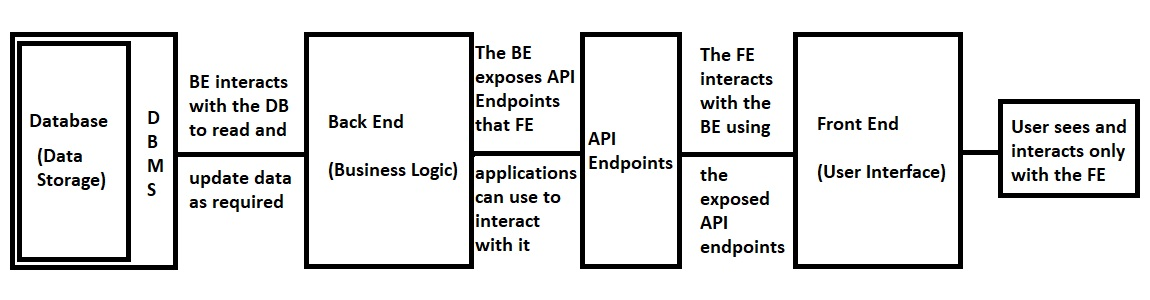
\includegraphics[width=15cm]{web-applications-architecture.jpg}
\end{figure}


\section{Database}
\subsection{Role of Database}
\paragraph{} The role of the database is to provide ways to the application to access and manipulate data. The database is accessed by Back End applications only. Front End cannot directly interact with the database.
\subsection{Database Options}
\paragraph{} The two most popular categories of databases are: 1. SQL and 2. NoSQL. For more on SQL databases \href{https://en.wikipedia.org/wiki/SQL}{click here} and for NoSQL \href{https://en.wikipedia.org/wiki/NoSQL}{click here}.
\paragraph{} Some popular SQL Databases:
\begin{itemize}
	\item Oracle Database
	\item Microsoft SQL Server
	\item MySQL
	\item PostgreSQL
	\item SQLite
\end{itemize}
\paragraph{} Some popular NoSQL Databases:
\begin{itemize}
	\item MongoDB
	\item Apache Cassandra
\end{itemize}


\section{Back End}
\subsection{Role of Back End}
\paragraph{} The role of the Back End is to implement the business logic of the application. It will expose API Endpoints which can be used by Front End applications. It is also responsible for the communication with the Database.
\subsection{Back End Options}
\begin{itemize}
	\item Java + Sprint Boot
	\item JavaScript + NodeJS + ExpressJS
	\item Python + Flask/Django
\end{itemize}
\subsection{Layers in Back End}
\paragraph{} I will use as example the architecture of a Java + Spring Boot Application.
\begin{itemize}
	\item \textbf{Database Layer:} The actual database (MySQL/MongoDB/Oracle SQL/etc).
	\item \textbf{Persistence Layer:} Responsible for Data Persistence. Consists of \textbf{Entities} and \textbf{DAOs}.
		\subitem \textbf{Entity:} a lightweight persistence domain object. Typically, an entity represents a table in a relational database.
		\subitem \textbf{Data Access Object (DAO):} is responsible for two concepts:
			\subsubitem One - Encapsulation of the details of the Persistence Layer and
			\subsubitem Two - Providing CRUD interface for a single entity.
			\subsubitem Note I: Persistence Layer (or else Repository Layer) is the layer that is responsible for data persistence, to access the cache and database.
			\subsubitem Note II: CRUD stands for Create-Read-Update-Delete.
	\item \textbf{Business Layer:} Contains all the business logic. It is responsible for  validation and authorization. Consists of \textbf{Services}.
		\subitem \textbf{Service:} -
	\item \textbf{Presentation Layer:} This is the top layer. It is responsible for handling HTTP requests and performing authentication. It is also responsible for handling the request (inputs) and the response.
		\subitem \textbf{Controller:} -
\end{itemize}
\subsection{Authentication vs Authorization}
\paragraph{} Authentication and Authorization are two different things.
\begin{itemize}
	\item \textbf{Authentication:} is the process of verifying who the user is.
	\item \textbf{Authorization:} is the process of checking if user is authorized to perform an action, i.e. retrieve some information, or delete some data.
\end{itemize}


\section{API}
\subsection{Role of API}
\paragraph{} The API will define the rules of communication between the Back End and the Front End applications.\\Note: API stands for Application Programming Interface.
\subsection{API Options}
\begin{itemize}
	\item REST
	\item SOAP
	\item WebSocket
	\item GraphQL
\end{itemize}


\section{Front End}
\subsection{Role of Front End}
\paragraph{} The Front End is the User Interface, it's what Users actually see and how they communicate with the Back End application. The Front End only communicates with the Back End applications via API calls.
\subsection{Front End Options}
\begin{itemize}
	\item HTML and CSS are common no matter the framework you chose
	\item TypeScript + Angular (Web Application)
	\item JavaScript + React (Web Application)
	\item TypeScript + Ionic (PWA Angular Based)
	\item JavaScript + Native (PWA React Based)
\end{itemize}
\paragraph{} Note: PWA stands for Progressive Web Application. It allows with a single code base, the application to run as web and android application at the same time. Android Users have the option to install the application like a normal android application however in reality it runs in browser in a standalone window instead of a browser tab.


\end{document}
